\documentclass[a4paper]{article}
%%% ATTENTION THIS DOCUMENT IS USING GITHUB FOR EDITING/CHANGING
%%%% DO GIT PULL BEFORE CHANGING ANYTHING
%%%% The reason it is like that is that ED will be doing some editing
%%%% on the plane over the next 24 hours

\usepackage{INTERSPEECH2015}

\usepackage{graphicx}
\usepackage{amssymb,amsmath,bm}
\usepackage{textcomp}
\usepackage{dsfont}
\usepackage{url}
\usepackage{color}


\def\vec#1{\ensuremath{\bm{{#1}}}}
\def\mat#1{\vec{#1}}
\newcommand{\set}[1]{\left\{#1\right\}}
\newcommand{\tup}[1]{\langle#1\rangle}
\newcommand{\N}{\mathbb{N}}
\newcommand{\card}[1]{\left\vert{#1}\right\vert}


\sloppy % better line breaks
\ninept



\title{A Hybrid Dynamic Time Warping-Deep Neural Network Architecture for Unsupervised Acoustic Modeling}
\makeatletter
\def\name#1{\gdef\@name{#1\\}}
\makeatother \name{{\em Roland Thiolli\`ere, Ewan Dunbar, Gabriel Synnaeve} \\
{\em Maarten Versteegh, Emmanuel Dupoux}}

\address{Ecole Normale Sup\'erieure / PSL Research University / EHESS / CNRS, France \\
  {\small \tt rolthiolliere@gmail.com, emd@umd.edu, gabrielsynnaeve@gmail.com} \\
  {\small \tt maartenversteegh@gmail.com, emmanuel.dupoux@gmail.com }
}


\begin{document}

\maketitle

%200 words max
\begin{abstract}
We report on an architecture for the unsupervised discovery of talker-invariant subword embeddings. It is made out of two components: a dynamic-time warping based spoken term discovery (STD) system and a siamese deep neural network (DNN). The STD system clusters word-sized repeated fragments in the acoustic streams while the DNN is trained to minimize the distance between time aligned frames of tokens of the same cluster, and maximize the distance between tokens of different clusters. We use additional side information regarding the average duration of phonemic units, as well as talker identity tags. For evaluation we use the data sets and metrics of the Zero Resource Speech Challenge. The model shows improvement over the baseline in subword unit modeling. 
\end{abstract}
\noindent{\bf Index Terms}: zero resource speech challenge, feature extraction, deep learning\let\thefootnote\relax\footnote{* These authors contributed equally to this work.}


\section{Introduction and rationale}
The automatic discovery of linguistic units from the raw speech stream \cite{XXX} may seem to be a daunting task from a scientific and technological point of view. Yet, the fact that infants spontaneously converge on what amounts to a functional speech recognizer (language-tuned acoustic and language models) within a year or so, by mere immersion in a linguistic community, indicates that it is not an impossible one. Certainly, infants do not construct a speech recognizer by being fed hours of speech paired with phone labels. However, their task is not totally unsupervised either. Apart from the fact that infant speech input is accompanied by multimodal signals that may contain relevant side information (visual context, social signals etc.), the speech signal itself is produced by an adult linguistic system which has a particular universal structure that the infant learner could exploit. Here, we will exploit one such source of information, related to the fact that speech contains hierarchically organized levels of structures: utterances are made of words, and words are made of phonemes. 

In particular, our paper rests on two critical assumptions regarding words and phonemes: (1) word classes are more separated in acoustic space than phoneme classes, (2) pairs of word tokens share most of their phonemes if they belong to the same class, and differ in most of their phonemes if not. At a high level, this suggests the following learning strategy: start by discovering word-like units from the signal using Spoken Term Discovery  (assumption 1), then, use the discovered word-like units to construct a phonetic tutor that trains phoneme-like representations (assumption 2). The phonetic tutor works by aligning each pair of word-like tokens and declaring that the aligned frames represent the same phonemes when the word-like tokens are in the same class, and different phonemes when they are in different classes. Here, we will apply this logic at the frame rather than the phone level, but the output of learning is still abstract speech features. We learn these using a deep neural network (DNN) architecture.

These two assumptions are easy to verify. For example, under a unigram model of the lexicon, in which each word is made up of random and independent draws from the phoneme inventory, it is easy to see that the acoustic overlap of two strings of phonemes will diminish with the size of the strings. As for the second assumption, the edit distance between two random words is high (using the normalized edit distance of \cite{XXX}, around .9, assuming a unigram lexicon with the phoneme distribution of English). With real lexicons, the unigram model does not hold, but these assumptions are still generally met, as illustrated in Figure 1. [XXX]

### XXX ###
#### XXX ###
In addition to exploiting the relationships between phonemes and words, our paper exploits two other potential sources of side information. The first one is that speech not only conveys linguistic information, but also information pertaining to talker identity. Here, we assume that talker identity is accessible to infants, either through an analysis of the speech signal alone (as in talker diarization) or using multimodal input. We will explore the fact that having access to talker ID information is useful, since it provides information about what information to \emph{ignore} or \emph{normalize for} in the speech signal. The second source of information could be an innate knowledge of the temporal properties of phoneme units in human languages. Typically phonemes have a duration around 70ms, and is most of the time comprised between 20ms and 200ms. One could use this source of knowledge to either discard sections of speech that are corrupted and therefore do not obey this structure, or to discard potentially flawed features representations for speech.
#### XXX ###
### XXX ###

Previous work in the psycholinguistic literature has shown that lexical information can help in discovering phoneme identity. Using a Bayesian model, Feldman et al.~\cite{XXX} demonstrated the feasibility of this principle in a toy model with simple Gaussian data. Martin et al.~\cite{XXX} and Fourtassi et al.~\cite{XXX} demonstrated using transcribed speech that such top down information can help to cluster allophones into phonemes. Synnaeve et al.~\cite{XXX} showed that, using oracle word labels, a deep neural network can be trained to yield a phonetic embedding whose performance on cross talker phoneme discrimination improves substantially on the raw input features. This architecture, {\sc ABnet}, is described below. Finally, Jansen et al.~\cite{XXX}, using an architecture on denoising auto-encoders, found that both oracle word labels and speech fragments discovered automatically can yield good speech features. Here we test whether the ABnet architecture can be coupled with a spoken term discovery system to yield synergistic learning in both directions (using words to help discovering phonemes and vice versa). 

### XXX ###
### XXX ###
As for using talker information as a side, there is a very rich literature in the HMM framework in talker normalization using feature or model transformation (cite). With DNN architecture, there is relatively less work, although a common technique consist in concatenating a speaker embedding (ie i vectors) with the input features during the training of network. (cite). Whether such technique will work in the context of a weekly supervised ABnet remains to be seen. Finally, regarding the temporal structure of phonemes, several papers have used the difference in autocorrelation between adjacent frames and distant frames as a measure of the quality of a speech recognizer (cite). The so called M or MDelta measure indeed predicts phone error rate, gowever has not up to our knowledge been used in the context of wealy supervized learning.
### XXX ###
### XXX ###

\section{System}
The entire system is presented in Figure \ref{XXX}. It is composed of several elements which we describe here. 

\subsection{Spoken term discovery}

We use the optimized JHU spoken term discovery system based on \cite{jansen}. The basic idea is to search for repeated acoustic patterns using dynamic time warping across the entire similarity matrix \cite{park}. Typically, repeated patterns show up as diagonal stretches of high similarity, which are then segmented out and fed into a clustering algorithm. The search is made tractable through the use of locality sensitive hashing, a technique using random vector projections followed by bit quantization. (Speech features that are initially vectors of floats in $d$ dimensions become vectors of bits in $b$ dimensions, for which the Hamming distance turns out to be an efficient approximation of the frame-wise cosine similarity metric.) The LSH bit signatures of each frame are sorted and scanned using a fixed width beam in order to restrict the computation of the frame-wise similarities to pairs of frames that are the most similar. This results in a sparse similarity matrix over the entire corpus. The similarity matrix is searched for diagonal patterns, and the algorithm outputs pairs of matched fragments together with their DTW score (the average similarity along the matching path). Further post processing involves recomputing the DTW scores using the real cosine function on the original input features, and applying connected component clustering of the found fragments, as in \cite{park}, in order to construct classes. In this paper, we used the implementation of \cite{jansen}, with an LSH similarity threshold of .5, a DTW threshold of .98, and a connected component threshold of .98. These numbers are the same as in \cite{XXX}, submitted, so that a comparison can be made.

\subsection{Phonetic tutor}

The phonetic tutor takes as input a list of matching word-like fragments and a frame-wise feature representation of these fragments. It outputs a list of matching and mismatching frames.

### XXX ###
For matching frames, it aligns each fragment pair using DTW with cosine distance on the feature representations, and returns each frame pair on the DTW path.

For mismatching pairs, it samples word fragment pairs belonging to different classes and aligns them using a diagonal line and returns each pair along it.
### XXX ###

Instead of taking all possible pairs of mismatching word fragments, our phonetic tutor undersamples them, first, in order to have the same number of matching as mismatching word pairs, and second, to balance the matching and mismatching word pairs to have both same-talker pairs and different-talker pairs. (The ratio of same to different talker was left free to vary depending on the input fragments.) This avoids a statistical bias in which the information about matching versus mismatching phonetic content is accidentally correlated with same versus different talker (which would turn the task into an easier talker ID task).

\subsection{ABnet}

\begin{figure}[h]
    \begin{center}
        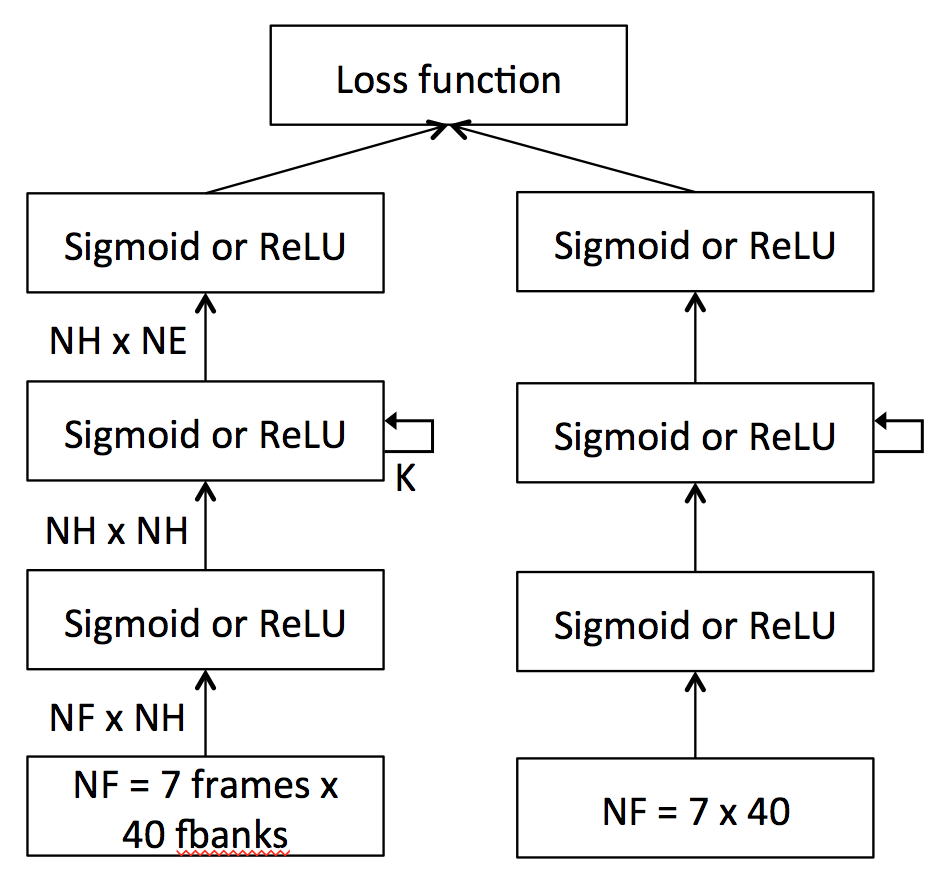
\includegraphics[width=0.68\columnwidth]{abnet}
        \caption{Schema of our siamese neural network. In the results presented here, we used varying K values (depth in hidden layers), NF=7, NH=500, NE=100 and sigmoid units.}
    \end{center}
    \label{fig:abnet}
\end{figure}


This part of the system learns a phonetic embedding, i.e., a vector representation of speech sounds. It is based on the work of \cite{synnaeve&dupoux2014}. Here we use a siamese network architecture \cite{siamese} (see Figure~\ref{fig:abnet}) where we stack 7 frames of input features in the input layer (a center frame, and 3 context frames on each side), followed by K layers of 500 units, and a final output layer of 100 units. Two identical copies of the same network are fed by the members of each pairs of features $A$, and $B$, respectively. %The output of these two networks ($y_A$ and $y_B$) are then compared using the $coscos^2$ loss function as follows:
%\begin{equation}
%\mathcal{L}(A,B) = w.(1-\cos(y_{A}, y_{B})) + (1-w).\cos^2(y_{A}, y_{B})
%\end{equation}
These are then forward propagated in the ABnet, where we finally use an asymmetric loss as found in \cite{drlim} for learning invariants in images, with a margin as in \cite{wsabie}. So that in the embedding (noted $Y$) we get:
\begin{eqnarray*}
    \mathcal{L}_{\textsc{coscos2}}(A,B) = \left\{
        \begin{array}{l}
              (1-\cos(Y_A, Y_B)) / 2 \ \ \ if\ \mathrm{same}\\
                \cos^2(Y_A, Y_B)\ \ \ if\ \mathrm{different}
            \end{array}\right.
        \end{eqnarray*}
        with $$\cos(x, y) = \frac{\langle x, y \rangle}{\|x\|\|y\|}$$


Over a whole batch, as we perform negative samples at a positive:negative rate of 1:1, this boils down to a loss of:
$$\mathcal{L}(A,B,C) = \frac{1 - \cos(Y_A, Y_B)}{2} + \cos^2(Y_A, Y_{C})$$
%with $w \in \{0,1\}$ (different or same word).
Roughly speaking, the loss function is minimum when the vector representations for matching frames are colinear for matching frames and orthogonal for mismatching frames. \textcolor{red}{TODO: Here it's maybe good to precise how same/diff apply to frames from spoken terms or close/far with MDelta} This $\textsc{coscos2}$ loss was shown to perform well in \cite{synnaeve}. The network is initialized with random weights and then trained on \textcolor{red}{TODO}\% of the data. The rest of the data is used as a heldout validation set, which is tested to stop training in order to prevent the network from overfitting. The  'early stopping' rule is \textcolor{red}{TODO}. The networks were trained for a maximum of 500 epochs by mini-batch stochastic gradient descent (using Adadelta \cite{adadelta}) on an Nvidia K20 Tesla GPU. The ABnet code uses the Theano library\cite{theano2010,theano2012}, and is freely available$^1$\footnote{1: \url{https://github.com/SnippyHolloW/abnet/}}.

\subsection{Mdelta filter}

XXX
The Mdelta measure that we used was based on hermaksnly. It uses a correlation method to derive two distance
XXX

\subsection{Talker ID}

XXX
Talker ID was just read off the filenames of both datasets. To derive the talker ID embedding, we used the same ABnet architecture and similar tutor, except that we used a cost function trying to optimize talker discrimination, across and withing phoneme identity.
XXX

\subsection{Speech features}

We use two sets of speech features. The FDLP features consist of a 5-dimensional XXXX with first and second derivatives, resulting in a 15 dimensional vector. These features have been shown to be resistant to talker change \cite{XXX}. The filterbank (FB) features are obtained by passing the signal through a 40-channel mel-scaled filterbank and applying cubic root compression. Both sets of features were mean-variance normalized file by file, skipping the areas indicated as non speech by the VAD.  [XXX - WHAT VAD]


\section{Experiments}


\subsection{Corpora}

We use the two corpora available from the ZeroSpeech2015 Challenge website (English and Xitsonga). 
The data sets are composed of selected segments from two free and open-access data sets: the Buckeye Corpus
of American English \cite{XXX} and the NCHLT Speech Corpus of the South African Languages \cite{XXX}. The English corpus consists of casual conversational speech from twelve speakers (between 16 and 30 minutes of speech each) for a total of about 5 hours. The Xitsonga corpus consists of read speech recorded by 24 speakers (12 male, 12 female). From each speaker, between 2 and 29 minutes were selected ($\mu=13.16$) with the same criteria as for the Buckeye corpus, for a total of 5h22m03s. For both corpora, the selected segments were provided to the participants and the remaining portions of the corpus were declared non-speech. Each segment or file contained speech for only one speaker and this information, as well as the speaker ID, was also provided. (The evaluation was based on forced aligned intervals for the phonemes in the corpora, but the forced alignments were not communicated to the participants.)

\subsection{Metrics}

We use the metrics from both Track 1 (subword unit discovery) and Track 2 (spoken term discovery). The Track 1 evaluation consists of an aggregate minimal pair ABX discrimination score run on all of the triphones of the given dataset. These scores indicate the separability in the embedding space of the phoneme classes, both within-talker and between-talker. The metrics of Track 2 include matching and clustering speech fragments and using them to parse the speech stream. 

\subsection{The base experiment: STD--DNN--STD}

\section{Experiments}

\subsection{Corpora}


The system ...

### XXX
\subsection{M-Delta filtering}
\subsection{Talker embedding normalization}
We use the previously described ABnet to output a talker embedding in 100 dimensions for each frame. We average those embeddings for each speaker and do an ICA to reduce the number of dimensions to 20. 
## XXX

\subsection{Improving word discovery: STD--DNN--STD}

The system ...

\section{Results}
This feature representation is then evaluated using the Track 1 ABX evaluation metrics and is shown in Table 1.
As seen, the results are quite good compared to the topline resuts. The distance used in the Track 1 metric is the symmetric KL-divergence.

\section{Discussion}
% tuned parameters:
% -complexity of the ABnet (although is does not matter that much)
% -std thresholds for ABnet best run
% -


\begin{table}[htb]
\caption{\label{tab:track1} {\it Within and across talker Minimal Pair ABX error rates for the Zerospeech Baseline (MFCC) and Topline (supervised HMM-GMM posteriorgrams), and for our systems.}}
\vspace{1mm}
\centerline{
\begin{tabular}{lcccc}
\hline
\vspace{1mm}        & \multicolumn{2}{c}{\underline{English}}  & \multicolumn{2}{c}{\underline{Tsonga}}    \\
                        & Within  & Across   & Within  & Across   \\
\hline
Baseline           & 15.6      & 28.1      & 19.1      & 33.8      \\
Our system1         & 00.0      & 00.0      & 00.0      & 00.0      \\
Our system2         & 00.0      & 00.0      & 00.0      & 00.0      \\
Our system3         & 00.0      & 00.0      & 00.0      & 00.0      \\
Topline            & 12.1      & 16.0      & 3.5       & 4.5      \\
\hline
\end{tabular}
}
\end{table}


%
%\setlength{\tabcolsep}{4pt}
%\begin{table*}[t]
%\begin{tabular}{lccccccccccccccccc}
%\hline
%         &       &       &\multicolumn{3}{c}{\underline{Matching}}&\multicolumn{3}{c}{\underline{Grouping}}&\multicolumn{3}{c}{\underline{Type}}&\multicolumn{3}{c}{\underline{Token}}&\multicolumn{3}{c}{\underline{Boundary}}\\
%         & NED   & Cov   & P        & R     & F       & P     & R     & F     & P     & R     & F     & P     & R     & F  & P     & R     & F    \\
%\hline
% &\multicolumn{17}{c}{\underline{English}}  \\
%Baseline & 0.219 & 0.163 & 0.394    & 0.016 & 0.031   & 0.214 & 0.846 & 0.333 & 0.062 & 0.019 & 0.029 & 0.055 & 0.004 & 0.080 & 0.441 & 0.047 & 0.086 \\
%Our system  & 0.000 & 0.000 & 0.000    & 0.000 & 0.000   & 0.000 & 0.000 & 0.000 & 0.000 & 0.000 & 0.000 & 0.000 & 0.000 & 0.000 & 0.000 & 0.000 & 0.000 \\
% &\multicolumn{17}{c}{\underline{Tsonga}}  \\
%Baseline & 0.120 & 0.162 & 0.691    & 0.003 & 0.005   & 0.521 & 0.774 & 0.622 & 0.032 & 0.014 & 0.020 & 0.026 & 0.005 & 0.008 & 0.223 & 0.056 & 0.089 \\
%Our system  & 0.000 & 0.000 & 0.000    & 0.000 & 0.000   & 0.000 & 0.000 & 0.000 & 0.000 & 0.000 & 0.000 & 0.000 & 0.000 & 0.000 & 0.000 & 0.000 & 0.000 \\
%\hline
%\end{tabular}
%\end{table*}
\bibliography{mybib}
\bibliographystyle{IEEEtran}

 \section{Acknowledgements}
RT, ED, GS, MV and ED's research was funded by the European Research Council (ERC-2011-AdG 295810 BOOTPHON), the Agence Nationale pour la Recherche (ANR-2010-BLAN-1901-1 BOOTLANG) and the Fondation de France. It was also supported by ANR-10-IDEX-0001-02 PSL and ANR-10-LABX-0087 IEC.


\end{document}
